\documentclass{article}

% ---------- Fonts & Encoding ----------
\usepackage[T1]{fontenc}
\usepackage[utf8]{inputenc}
\usepackage{lmodern}
\usepackage{microtype}

% ---------- Math, Figures, Tables ----------
\usepackage{amsmath, amssymb}
\usepackage{graphicx}
\usepackage{booktabs}
\usepackage{multirow}
\usepackage{overpic}
\usepackage{siunitx}

% ---------- Captions ----------
\usepackage{caption}
\usepackage{subcaption}

% ---------- Colors (before hyperref) ----------
\usepackage{xcolor}

% ---------- DLAI Style (optional) ----------
% If the style file exists, load it; otherwise define minimal fallbacks.
\makeatletter
\@ifpackageloaded{dlaiml2025}{}{%
  \IfFileExists{dlaiml2025.sty}{%
    \usepackage[accepted]{dlaiml2025}%
  }{%
    % Minimal fallbacks so the document still compiles without dlaiml2025.
    \newcommand{\dlaititlerunning}[1]{}%
    \newcommand{\dlaititle}[1]{\title{#1}}%
    \newenvironment{dlaiauthorlist}{}{}%
    \newcommand{\dlaiauthor}[2]{}%
  }%
}
\makeatother

\usepackage{hyperref}

\dlaititlerunning{Geodesic Post-Hoc Quantization for VAEs}

\begin{document}

\setlength{\parskip}{0pt plus 0.2pt minus 0.2pt}


\twocolumn[
\dlaititle{Geodesic Post-Hoc Quantization for Variational Autoencoders}

\begin{dlaiauthorlist}
\dlaiauthor{Marco Galletti (2109043)}{sapienza}
\end{dlaiauthorlist}

\dlaiaffiliation{sapienza}{Sapienza University of Rome}

\dlaicorrespondingauthor{Marco}{galletti.2109043@studenti.uniroma1.it}

\vskip 0.3in
]

\printAffiliationsAndNotice{}

\begin{abstract}
This project revisits the classic VQ-VAE by implementing a post-hoc quantization pipeline.
This work compares an end-to-end trained VQ-VAE against a post-hoc method that uses a novel geodesic clustering algorithm based on a metric derived from the VAE decoder's geometry on the CIFAR-10 dataset. 
The results reveal that the inherent "training mismatch" of the proposed framework proves to be a significant bottleneck, with the VQ-VAE achieving superior results across all metrics. 
\end{abstract}

\section{Introduction}
Generative models, particularly Variational Autoencoders (VAEs), are powerful tools for learning low-dimensional representations of complex data. 
The Vector Quantized VAE (VQ-VAE) extends this by learning a discrete latent space, which is often more suitable for downstream tasks such as autoregressive modeling.
Standard VQ-VAEs learn this discrete representation end-to-end with the encoder and decoder.
This work explores an alternative quantization pipeline, where a continuous-latent VAE is first trained,
and a discrete codebook is then built by applying clustering algorithms to its latent space. 
The primary contribution is the implementation and evaluation of a geometrically-motivated a posteriori quantization method on the CIFAR-10 dataset, comparing it directly against a standard VQ-VAE to investigate the trade-offs between these two paradigms.

The code for this project is available at \url{https://github.com/m4rch1n0/vqvae}.

\section{Related Work}
The project builds upon three main areas of research: discrete latent variable models, the geometric analysis of latent spaces, and graph-based clustering methods.

\paragraph{Discrete Latent Representations.} The VQ-VAE \cite{van2017neural} is the foundational model for learning discrete representations for generative tasks. 
It introduces the paradigm of learning a discrete codebook with the encoder and decoder, and uses a powerful autoregressive model over the resulting spatial grid of codes to generate high-fidelity images. 
The research in this project deliberately deviates from this by exploring a post-training quantization scheme, which separates the continuous representation learning from the codebook creation.

\paragraph{Geometry of VAE Latent Spaces.} The core motivation for the geodesic method comes from works that model the latent space of a VAE as a Riemannian manifold. Arvanitidis et al. \cite{arvanitidis2017latent} established the use of the pull-back metric tensor, defined by the decoder's Jacobian ($M(z) = J(z)^T J(z)$), to better represent the geometry of the data manifold. They argued for using geodesic distances, rather than Euclidean ones, for tasks like interpolation and clustering. Shao et al. \cite{shao2018riemannian} further developed practical methods for geodesic computation, though they noted that for some image VAEs, the learned manifolds can be nearly flat, making Euclidean distance a reasonable approximation. 
This work leverages these geometric insights directly, using Jacobian-vector product to approximate local geodesic distances for clustering.

\paragraph{Graph-Based Geodesic Approximation.} The specific technique of approximating geodesic distances by computing shortest paths on a k-Nearest Neighbors (k-NN) graph was popularized by Isomap \cite{tenenbaum2000global} in the context of manifold learning. This approach provides a computationally feasible way to estimate global manifold distances from local neighborhood information. The methods presented here are a direct application of this principle: a k-NN graph is constructed and shortest-path distances (via Dijkstra's algorithm) are used as the metric for the k-medoids clustering algorithm, with the key novelty being the re-weighting of the graph's edges with the learned Riemannian metric.

\section{Method}
The pipeline consists of three main stages: continuous representation learning, post-hoc quantization, and autoregressive modeling.

\subsection{Model Architectures\protect\footnote{Model implementations are available at \texttt{vqvae/src/models/}. The vanilla VAE used in the Appendix is also available here.}}
\paragraph{Spatial VAE.} The VAE encoder consists of three convolutional layers (with 64, 128, and 256 channels respectively, stride 2, and Batch Normalization) that downsample the input image to a $4 \times 4$ spatial grid. 
Two final $1 \times 1$ convolutions produce the mean and log-variance for a 32-dim latent space at each spatial location. The decoder mirrors this architecture using transposed convolutions to reconstruct the image.

\paragraph{Transformer.} A decoder-only Transformer is used for autoregressive modeling of the quantized latent codes. The model has 4 layers, 4 attention heads, an embedding dimension of 256, and is trained on flattened $16$-token sequences.

\subsection{Training Details}
The \texttt{SpatialVAE} was trained for 200 epochs using the AdamW optimizer with a learning rate of $10^{-3}$, a weight decay of $10^{-5}$, and a cosine learning rate schedule. The Transformer model was also trained for 200 epochs with AdamW, but with a learning rate of $3 \times 10^{-4}$ and a weight decay of $0.01$. The batch size was 256.

\subsection{Post-Hoc Quantization Method}
After training the VAE, the mean latent vectors ($\mu$) are extracted from the training set and a discrete codebook is built using a geometrically rigorous clustering scheme. This is the \textbf{Full Riemannian Geodesic Clustering} method. The process is as follows:
\begin{enumerate}
    \item \textbf{k-NN Graph Construction:} A k-Nearest Neighbors graph (with k=50) is constructed from the flattened latent vectors to establish local connectivity.
    \item \textbf{Riemannian Re-weighting:} \textit{All} unique edges in this graph are re-weighted using a metric derived from the VAE decoder's geometry, approximated via efficient Jacobian-vector products.
    \item \textbf{Geodesic K-Medoids:} K-Medoids clustering (with K=512) is performed on the re-weighted graph. Distances are computed as the shortest paths on the graph using \textbf{Dijkstra's algorithm}, and the process is initialized with a K-Means++ strategy. Clustering is performed on the largest connected component (LCC) of the graph to ensure all points are mutually reachable.
\end{enumerate}

\subsection{Autoregressive Modeling}
Once the codebook is built, the spatial latent grids for each training image are quantized, converting them into sequences of discrete integer codes. A decoder-only Transformer model is then trained to predict the next code in a sequence, \textbf{conditioned on the previous ones}. This allows for autoregressive generation of novel sequences of codes, which can then be mapped back to latent vectors via the codebook and rendered into images by the VAE decoder.

\section{Experiments and Results}
The evaluation was performed on the CIFAR-10 dataset. Performance was assessed using Peak Signal-to-Noise Ratio (PSNR), Structural Similarity Index (SSIM), and Learned Perceptual Image Patch Similarity (LPIPS).


The results (Table~\ref{tab:cifar10_results}) suggest the superiority of the end-to-end approach, which outperforms the post-hoc method across all key metrics.
This suggests the solidity of jointly training the encoder, decoder, and codebook on complex data distributions.

\begin{table}[h!]
\caption{CIFAR-10 Method Comparison.\protect\footnotemark}
\label{tab:cifar10_results}
\begin{center}
\begin{footnotesize}
\begin{tabular}{l c c c}
\toprule
Method & PSNR (dB) & SSIM & LPIPS \\
\midrule
Post-Hoc (Full Riemannian) & 8.72 & 0.005 & 0.564 \\
Baseline VQ-VAE & \textbf{9.49} & \textbf{0.019} & \textbf{0.475} \\
\bottomrule
\end{tabular}
\end{footnotesize}
\end{center}
\vspace{-0.4cm}
\end{table}
\footnotetext{Metrics are computed consistently across all methods. While absolute values may be implementation-dependent, the relative performance ranking is valid.}

\begin{figure}[ht!]
    \centering
    \begin{subfigure}[b]{0.49\columnwidth}
        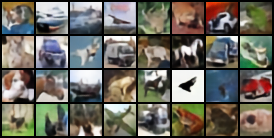
\includegraphics[width=\linewidth]{images/cifar10_baselineVQ.png}
        \caption{Baseline VQ-VAE (Reconstructions)}
        \label{fig:cifar_baseline}
    \end{subfigure}
    \hfill
    \begin{subfigure}[b]{0.49\columnwidth}
        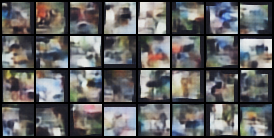
\includegraphics[width=\linewidth]{images/cifar10_spatial_geodesic_generated_samples.png}
        \caption{Post-Hoc Spatial Geodesic (Generated)}
        \label{fig:cifar_spatial}
    \end{subfigure}
    \caption{Qualitative comparison on CIFAR-10. (a) Reconstructions from the end-to-end VQ-VAE. (b) Samples generated by the Transformer in the post-hoc spatial geodesic pipeline.}
    \label{fig:cifar_recon}
\end{figure}

\section{Discussion and Conclusions}
On CIFAR-10, the "training mismatch" in post-hoc methods appears to create a performance bottleneck that is overcome by the joint, end-to-end optimization of a standard VQ-VAE.

In conclusion, this project reveals a complex trade-off between geometric fidelity and reconstruction performance. While leveraging a metric derived from the VAE decoder's geometry can substantially reduce latent-space quantization error (as detailed in the Appendix), this does not guarantee superior image quality on complex datasets. For CIFAR-10, the end-to-end trained VQ-VAE achieves superior results. Future work could address the limitation of the post-hoc approach by fine-tuning the VQ-VAE decoder on the discrete codebook, potentially combining the benefits of geometric clustering with the performance of a jointly-optimized system. A full comparative analysis on the simpler FashionMNIST dataset, which shows different performance characteristics, is provided in the Appendix.

\bibliography{references.bib}
\bibliographystyle{dlaiml2025}

\end{document}
